\documentclass[11pt]{article}
\usepackage{geometry}
\usepackage{amsmath, amssymb}
\usepackage{booktabs}
\usepackage{graphicx}
\usepackage{hyperref}
\usepackage{listings}
\usepackage{enumitem}
\usepackage{float}
\usepackage[colorinlistoftodos]{todonotes}
\usepackage{setspace}
\usepackage{iftex}
\usepackage{comment}
\usepackage[numbers]{natbib}
\ifPDFTeX
\renewcommand{\familydefault}{\sfdefault}
\else
\usepackage{fontspec}
\setmainfont{DejaVu Serif}
\fi
\usepackage{fancyhdr}
\geometry{
	paper=a4paper,
	top=3cm,
	bottom=2cm,
	left=2cm,
	right=2cm,
	headheight=2.5cm,
	footskip=1cm,
	headsep=0.2cm,
}
\hypersetup{colorlinks=true,linkcolor=black,citecolor=black,urlcolor=black,
            hypertexnames=false}
\onehalfspacing
\numberwithin{equation}{section}
\emergencystretch=2em
\graphicspath{{figs/}}

\definecolor{aicolor}{HTML}{6E2A8C}
\ifdefined\hideai
  \long\def\ai#1{}
\else
  \long\def\ai#1{{\color{aicolor}#1}}
\fi

\providecommand{\mnras}{MNRAS}
\providecommand{\aap}{A\&A}
\providecommand{\aapr}{A\&A Rev.}
\providecommand{\apj}{ApJ}
\providecommand{\apjs}{ApJS}
\providecommand{\apjl}{ApJ}
\providecommand{\araa}{ARA\&A}
\providecommand{\nat}{Nature}
\providecommand{\physrep}{Phys. Rep.}
\providecommand{\ssr}{Space Sci. Rev.}

% Metadata macros
\newcommand{\Class}{Specialized Topics of Theoretical Physics}
\newcommand{\Title}{Majorana Modes in the Machine – \\ Simulating Topological Phases with Quantum Circuits and AI}
\newcommand{\subtitle}{NISQ Noise on the Diagnostic}
\newcommand{\assignmentSemester}{SS 26}
\newcommand{\AuthorName}{Dobromir Stoev}
% TODO(Dobromir): replace this placeholder with your matriculation number.
\newcommand{\AuthorNumber}{TBD}
\newcommand{\FacultyName}{FAKULTÄT FÜR PHYSIK\\UND GEOWISSENSCHAFTEN}
\newcommand{\Supervisor}{\href{mailto:rosenow@physik.uni-leipzig.de}{Prof. Dr. Bernd Rosenow}}

\pagestyle{fancy}
\author{
    \textit{\Large\AuthorName}\\[4pt]
    \textit{\Large[ \AuthorNumber\ ]}\\
    \\ \\
    \textit{\Large Supervisor:\ \Supervisor}
}
\date{}
\title{
	\vspace{0.2\textheight}
	\textbf{\Huge\Class} \\ 
	\vspace{10pt}
	\textbf{\LARGE\Title} \\ 
	\vspace{10pt}
	\textbf{\Large\subtitle}
	\vspace{10pt}
}

\fancypagestyle{firstpage}{
    \fancyhead[L]{
\includegraphics[height=2cm]{uni_leipzig_logo.png}}
    \fancyhead[R]{\textsf{\Large \FacultyName} \\}
    \fancyfoot[L]{}
    \fancyfoot[C]{}
    \fancyfoot[R]{\textsf{\assignmentSemester}}
}
\pagestyle{fancy}
\fancyhead[L]{}
\fancyhead[R]{}
\fancyfoot[L]{}
\fancyfoot[R]{\small\thepage}
\fancyfoot[C]{}
\renewcommand\headrulewidth{0pt}

\begin{document}
\maketitle
\thispagestyle{firstpage}
\newpage
\tableofcontents
\newpage

% report body goes here with input block
% ============================================================================
% 00_intro.tex  --  Introduction  (~1/2 page)
%
% GOAL: State which of the six parts this report covers, why it matters, and
%       where it sits in the overall project. One paragraph of motivation, one
%       paragraph locating your part relative to the neighbouring parts (use a
%       one-line "see [Author, Part N]" cross-reference at each seam instead of
%       re-explaining a neighbour's material).
% Keep the whole report to 4-5 pages; this section is the shortest.
% ============================================================================

\section{Introduction}
\label{sec:intro}

The 1D Kitaev chain hosts unpaired Majorana zero modes at its ends in the
topological phase~\cite{kitaev2001}.
\ai{In the preceding part of the project, a parity-constrained variational
quantum eigensolver (VQE) prepared the finite-chain ground state and measured the
non-local edge string $O_{\mathrm{edge}}=X_0Z_1\cdots Z_{L-2}X_{L-1}$.  That
ideal result does not yet answer the experimentally relevant question: does the
diagnostic remain visible after imperfect gates, decoherence, readout errors,
and a noisy variational loop?}

\ai{This report covers Part 5, \emph{NISQ Noise on the Diagnostic}.  It isolates
noise at three different levels---a frozen state, the gates of the preparation
circuit, and the variational parameters---and then removes two simplifying
assumptions by optimizing the noisy cost and using a recorded backend calibration.
The emphasis is quantitative: the same $L=4$ circuit and edge-string observable
are retained while only the noise model or ansatz depth is changed.}

\ai{The noiseless construction of the VQE and string-measurement circuit belongs
to Zhengyi Liu's Part 4.  The symmetry-based taxonomy of physical Kitaev-chain
errors and the scaling to large $L$ belong to Edgar Harutyunyan's Part 6; here
$T_1/T_2$ enter only as device-level channels acting on the simulated circuit.}

% ============================================================================
% 10_theory.tex  --  Theory / derivation  (~1 - 1.5 pages)
%
% GOAL: The physics or derivation your part owns. Mine the matching notes/*.tex
%       listed for your part in ../../reports/README.md -- adapt and cite them,
%       do NOT re-derive from scratch. Equations use \numberwithin so they read
%       as (sec.eq).
% ============================================================================

\section{Noise model and diagnostic}
\label{sec:theory}

\subsection{Gate-level quantum channels}

\ai{An ideal gate $g$ acts on a density matrix as
$\mathcal U_g(\rho)=U_g\rho U_g^\dagger$.  In the circuit-level model the ideal
gate is followed immediately by a completely positive trace-preserving channel,}
\begin{equation}
  \widetilde{\mathcal U}_g=\mathcal E_g\circ\mathcal U_g,
  \qquad
  \mathcal E_g(\rho)=\sum_k K_k\rho K_k^\dagger,
  \qquad
  \sum_k K_k^\dagger K_k=I .
  \label{eq:kraus}
\end{equation}
\ai{For a circuit containing $M$ gates, the output is the ordered composition
$\rho_{\mathrm{out}}=(\mathcal E_{g_M}\!\circ\mathcal U_{g_M})\circ\cdots\circ
(\mathcal E_{g_1}\!\circ\mathcal U_{g_1})(\rho_0)$.  Noise therefore accumulates
with the actual transpiled gate count rather than being applied once to the final
state.  Qiskit Aer implements this construction with a density-matrix simulator
and a \texttt{NoiseModel}~\cite{qiskit2024}.}

\ai{The controlled baseline attaches a two-qubit depolarizing channel after
every \texttt{cx},}
\begin{equation}
  \mathcal E^{\mathrm{dep}}_p(\rho)
  =(1-p)\rho+p\,\frac{\operatorname{Tr}\rho}{2^n}I .
  \label{eq:depol}
\end{equation}
\ai{A second model uses gate-duration-dependent thermal relaxation.  For a gate
of duration $\tau$, amplitude loss has probability
$p_{T_1}=1-e^{-\tau/T_1}$, while $T_2$ controls the decay of off-diagonal
coherences.  The two mechanisms differ operationally: relaxation may move the
prepared state out of its target parity sector, whereas dephasing directly
suppresses the endpoint coherence needed by the edge string.  These are channel
mechanics only; their classification as physical errors of the Kitaev chain is
deferred to Part 6.}

\subsection{Three locations for error}

\ai{The study separates effects that can otherwise be confused.  The Week-8
\emph{frozen-state} test takes the validated state and applies readout or a single
post-preparation channel.  Symmetric assignment error $\epsilon$ attenuates a
weight-$L$ Pauli string as}
\begin{equation}
  \langle O_{\mathrm{edge}}\rangle_{\mathrm{readout}}
  =(1-2\epsilon)^L\langle O_{\mathrm{edge}}\rangle,
  \label{eq:readout}
\end{equation}
\ai{with an additional statistical uncertainty of order
$N_{\mathrm{shots}}^{-1/2}$.  The \emph{circuit-level} test instead applies a
channel after every entangling gate.  Finally, a coherent calibration error
replaces $\theta^*$ by $\theta^*+\delta\theta$ but keeps the state pure; an
incoherent channel generally lowers $\operatorname{Tr}\rho^2$.  Purity therefore
distinguishes a unitary miscalibration from genuine mixing even when both reduce
$|\langle O_{\mathrm{edge}}\rangle|$.}

\subsection{Expressibility versus accumulated noise}

\ai{For the linear-entanglement \texttt{EfficientSU2} ansatz, $r$ repetitions on
$L$ qubits contain $r(L-1)$ CNOTs.  A useful approximation to the measured
signal is}
\begin{equation}
 |\langle O_{\mathrm{edge}}\rangle|_{\mathrm{meas}}(r)
 \simeq
 |\langle O_{\mathrm{edge}}\rangle|_{\mathrm{ideal}}(r)
 (1-p_{\mathrm{cx}})^{r(L-1)} .
 \label{eq:depth_tradeoff}
\end{equation}
\ai{The first factor can have an expressibility threshold; the second decreases
at every added layer.  The relevant optimum is consequently the shallowest
depth that can represent the target state, not the deepest affordable circuit.}

\ai{Putting noise inside the VQE changes the objective itself.  With parity
$P=\prod_j Z_j$, the cost evaluated on the noisy density matrix is}
\begin{equation}
 C_{\mathrm{noisy}}(\theta)
 =\operatorname{Tr}[H\rho_\theta]
 +\lambda\bigl(1-\operatorname{Tr}[P\rho_\theta]\bigr)^2,
 \qquad
 \rho_\theta=\mathcal E\!\left(U(\theta)|0\rangle\langle0|U^\dagger(\theta)\right).
 \label{eq:noisy_cost}
\end{equation}
\ai{A lower value of Eq.~\eqref{eq:noisy_cost}, or even a larger noisy edge
string, need not imply a higher-fidelity ground state.  The re-optimized angles
must therefore be checked in a noiseless circuit against the exact ground state.}

% ============================================================================
% 20_results.tex  --  Methods & results  (~2 pages, the core of the report)
%
% GOAL: What you computed and what it shows. Include the key figure(s) for your
%       part ONLY (see the Code/figs column for your part in
%       ../../reports/README.md). Regenerate fresh PDFs with the block runner,
%       e.g.  python src/block1.py --plots 6   (venv /opt/python-envs/myenv),
%       and copy them into a local figs/ folder. Do NOT use showcase.py gallery
%       images (shared). Report concrete numbers, not just plots.
% ============================================================================

\section{Methods and Results}
\label{sec:results}

\subsection{Circuit-level implementation and verification}

\ai{All circuit results use a chain of $L=4$ sites, hopping strength $t=1$,
pairing strength $\Delta=1$, and the parity-constrained VQE and edge string from
Part 4.  The chemical potential $\mu$ is varied to cross the phase transition.
The preparation circuit contains single-qubit $R_Y$ rotations and linear CNOT
gates~\cite{peruzzo2014vqe}.  Before simulation it is written in the fixed gate
set \texttt{[rz,sx,cx]} without removing gates.  An error assigned to
\texttt{cx} therefore acts after every CNOT.  The output density matrix $\rho$
gives the edge-string value
$\operatorname{Tr}(O_{\mathrm{edge}}\rho)$.}

\ai{The implementation was checked with a separate calculation that applies
each gate and each depolarizing channel directly, without using Aer's noise
machinery.  Across 41 values of $\mu/t$, the two calculations differ by only
about $10^{-15}$.  Figure~\ref{fig:verification} also compares the deliberately
strong CNOT depolarizing strength $p_{\mathrm{cx}}=0.10$ with thermal relaxation
at $T_1=80\,\mu\mathrm{s}$, $T_2=60\,\mu\mathrm{s}$ and CNOT duration
$\tau_{\mathrm{cx}}=300\,\mathrm{ns}$.  The relaxation probability per gate is
only $1-e^{-\tau_{\mathrm{cx}}/T_1}\simeq0.0037$, so the thermal curve remains
closer to the ideal result.}

\begin{figure}[H]
  \centering
  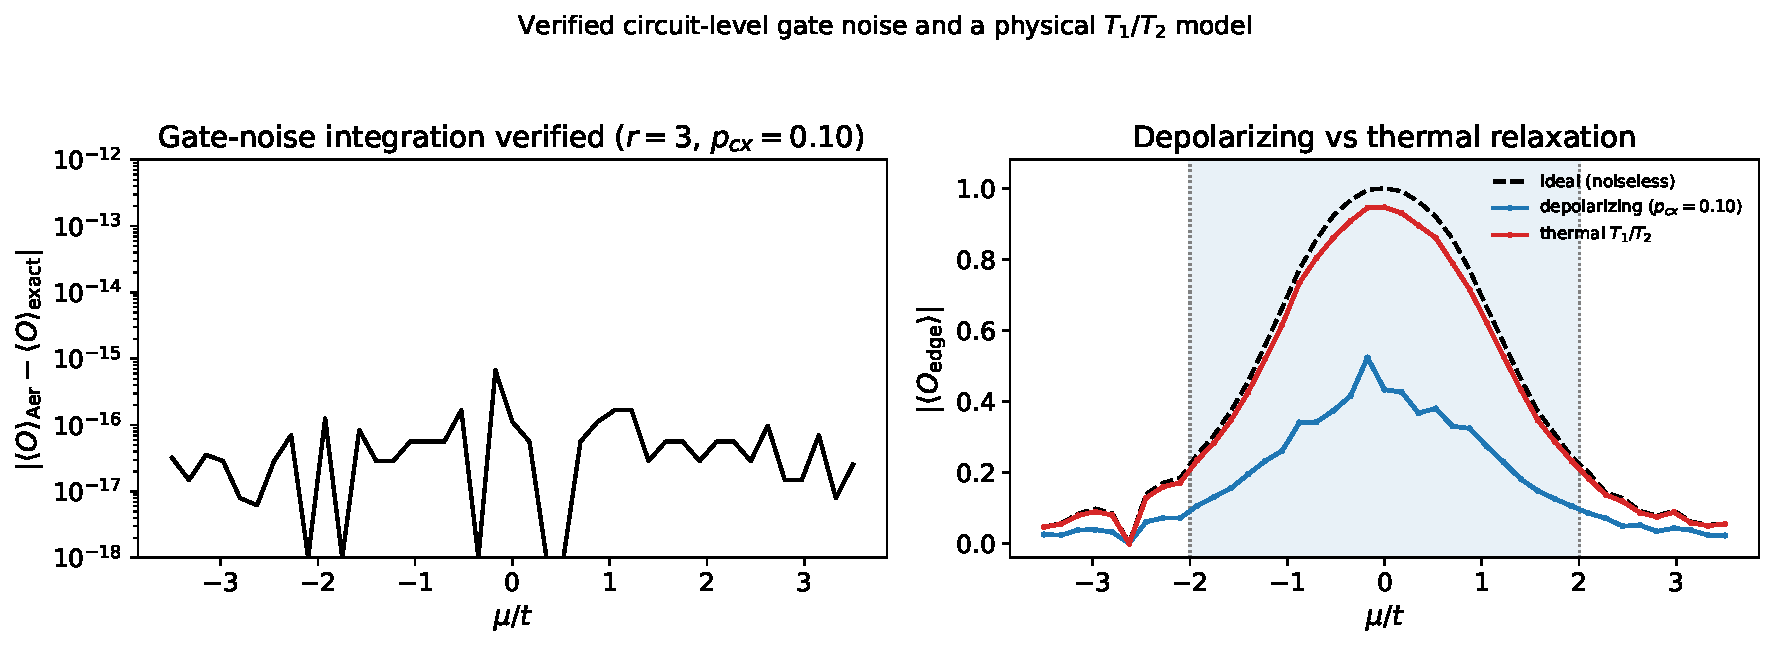
\includegraphics[width=0.98\linewidth]{block4_week9_verification.pdf}
  \caption{Left: the Aer \texttt{NoiseModel} edge string and the independent
  exact gate-by-gate reference agree to $\sim10^{-15}$ across the $\mu$ sweep.
  Right: depolarizing versus thermal $T_1/T_2$ noise at matched gate placement.}
  \label{fig:verification}
\end{figure}

\subsection{The optimal depth is an expressibility threshold}

\ai{At the topological sweet spot $\mu=0$, the noiseless edge string is only
$\simeq0.004$ for one repetition ($r=1$), but reaches approximately one at
$r=2$ and changes little in deeper circuits.  The first circuit is simply too
shallow to represent the state.  With $p_{\mathrm{cx}}=0.05$, the measured
signal peaks at $r^*=2$; every further repetition adds three noisy CNOTs without
improving the ideal state.  Figure~\ref{fig:depth} shows these two effects
separately.}

\begin{figure}[H]
  \centering
  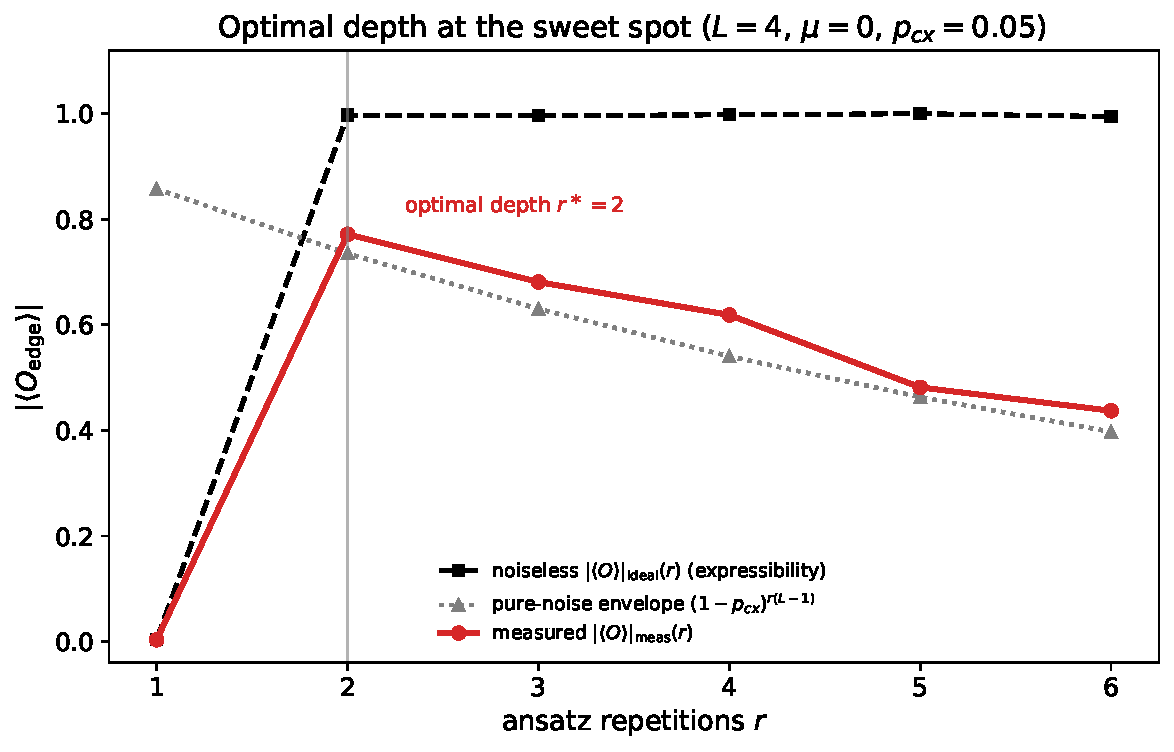
\includegraphics[width=0.72\linewidth]{block4_week9_depth_optimum.pdf}
  \caption{For $L=4$, the noiseless edge string has an expressibility threshold:
  $r=1$ fails, $r=2$ succeeds, and deeper circuits mainly accumulate CNOT noise.}
  \label{fig:depth}
\end{figure}

\ai{Angle errors provide a second check.  A random shift $\delta\theta$ rotates
the ideal state away from the optimum while its purity stays at one.  CNOT
depolarization reduces the same edge string while the purity falls.  The first
error can in principle be corrected by recalibrating the angles; the second
cannot be removed by changing one set of angles.}

\subsection{Noisy optimization and backend calibration}

\ai{This experiment fixes $r=3$, which does not replace the $r=2$ optimum found
above.  The earlier test asks which depth gives the largest measured signal for
$p_{\mathrm{cx}}=0.05$.  Here the purpose is different: the depth is held fixed
one layer above the representation threshold so that only the response of the
optimizer to two noise channels is compared.  Thus $r=3$ is a controlled test
setting, not a recommended operating depth; its extra CNOTs also explain why its
absolute noisy values are lower than an $r=2$ run would be.}

\ai{The noisy-cost calculation uses $L=4$, $r=3$, $\mu=0$, parity-penalty
strength $\lambda=0.1$, and the COBYLA optimizer.  It starts from the noiseless
angles and also tries several random starting points.  A channel is
\emph{unital} if it leaves the fully mixed state unchanged; it does not pull the
system toward one preferred state.  Depolarizing noise is unital, and optimizing
again changes the result very little.  A \emph{non-unital} channel does prefer a
state.  Amplitude damping is non-unital because it drives qubits toward
$|0\rangle$.  Under this channel, re-optimization can increase the
\emph{measured} edge string while moving the corresponding noiseless circuit
away from the exact ground state.  Table~\ref{tab:noisy} gives selected values
from the seed-7 sweep.}

\begin{table}[H]
  \centering
  \small
  \begin{tabular}{llcccc}
    \toprule
    channel & strength & \multicolumn{2}{c}{$|\langle O_{\mathrm{edge}}\rangle|$ noisy}
      & \multicolumn{2}{c}{fidelity to exact GS}\\
    \cmidrule(lr){3-4}\cmidrule(lr){5-6}
      & & fixed $\theta^*$ & noise-aware & fixed $\theta^*$ & noise-aware\\
    \midrule
    depolarizing & $0.08$ & $0.502$ & $0.501$ & $0.998$ & $1.000$\\
    amplitude damping & $0.08$ & $0.422$ & $0.565$ & $0.998$ & $0.994$\\
    amplitude damping & $0.12$ & $0.266$ & $0.337$ & $0.998$ & $0.966$\\
    \bottomrule
  \end{tabular}
  \caption{Best-case versus noise-aware optimization at $L=4$, $r=3$, $\mu=0$.
  Under amplitude damping the measured edge string rises while the noiseless
  fidelity to the exact ground state falls at strong damping.}
  \label{tab:noisy}
\end{table}

\ai{Finally, \texttt{NoiseModel.from\_backend} replaces the uniform test channel
with a recorded \texttt{FakeManilaV2} calibration.  Its CNOT error rates vary
from about $0.009$ to $0.014$.  At $\mu=0$ the ideal, backend-calibrated, and
uniform $p_{\mathrm{cx}}=0.05$ edge strings are $0.99$, $0.87$, and $0.67$.
The uniform model is therefore a deliberately harsh comparison, not a device
prediction.  The backend result is still optimistic: its readout errors are not
used because the simulation evaluates
$\operatorname{Tr}(O_{\mathrm{edge}}\rho)$ without measurement instructions.
The data also come from a recorded calibration, not a live hardware run.}

\ai{Together these tests show that realistic noise primarily reduces the
contrast of the non-local diagnostic.  Circuit depth should be chosen by
noiseless expressibility validation followed by noisy evaluation, and any
noise-aware optimization must report a state-quality check rather than only the
observable it was able to improve.  These conclusions concern the $L=4$ NISQ
circuit; their large-$L$ consequences are treated separately in Part 6.}

% ============================================================================
% 30_ai.tex  --  AI-collaboration note  (~1/3 page)
%
% GOAL: A short, honest reflection on how LLMs were used as a research
%       collaborator for this part (what they helped derive/debug/write, and
%       where you corrected them). This is a course requirement of the
%       AI-augmented seminar.
% ============================================================================

\section{On the AI collaboration}
\label{sec:ai}

My experience using large language models throughout the project was generally
positive.  We used Anthropic's Claude Opus 4.8 through Claude Code and OpenAI's
GPT-5.6 Sol through Codex CLI.  The models helped us to prepare the weekly presentations,
write topic-specific notes, and solve the main coding challenges.  They proved to be helpful as
editors and as personal physics teachers, especially when generating all the learning materials.  In addition, a collaborative GitHub repository and regular
group meetings also contributed to a professional working environment.  The
project inspired me to learn more about quantum computing and recent
developments in topological quantum computers.


\newpage
\bibliographystyle{plainnat}
\bibliography{references}

\end{document}
